% !TEX root = rapport_root.tex
\section{Analysis using projections}
The following sections outlines the use of the previously described 2D projection scoring to analyze, classify and interpret patterns among theoretical frameworks published in physics education research, utilzing the ChatGPT-sorted dataset containing $\sim$600 "Theory" sections, divided into $\sim130$ seperate categories.

\subsection{Category Grouping using Centroid Difference Vectors}
\noindent Attempting to divide these $\sim130$ seperate categories into two superordinate classes, we identify two rough overarching categories
\begin{enumerate}
    \item Cognitive, Conceptual and Mathematical Theories.
    \item Critical Theories concerning Social Justice, Identity and related constructs.
\end{enumerate}
Mean embeddings for each were calculated using the frameworks "Philosophy of Science", "Mathematical Modeling", "Conceptual Change Theory", "Cognitive Load Theory" and "Communities of Practice", "Critical Race Theory" and "Sociocultural Identity Frameworks", respectively. Taking the vector difference of these centroids and projecting all samples against it, we see a rough clustering (see \Cref{fig:109}). The right hand side of the plot contains theories such as "Culturally Relevant Pedagogy", "Gender Performativity" and "Quantitative Critical Race Theory", while the left side is mostly inhabited by different conceptual theories such as "Conceptual Blending Theory" and "Conceptual Metaphor Theory", as well as "Measurement Theory", "Epistemic Games" and "Math-Physics Algorithmic Theory". The middle ground is occupied by "Activity Theory", "Argumentation Theory" and "Intellectual Humility Framework" which perhaps do not fit very well into either category.

\begin{figure}%[h]
    \centering
    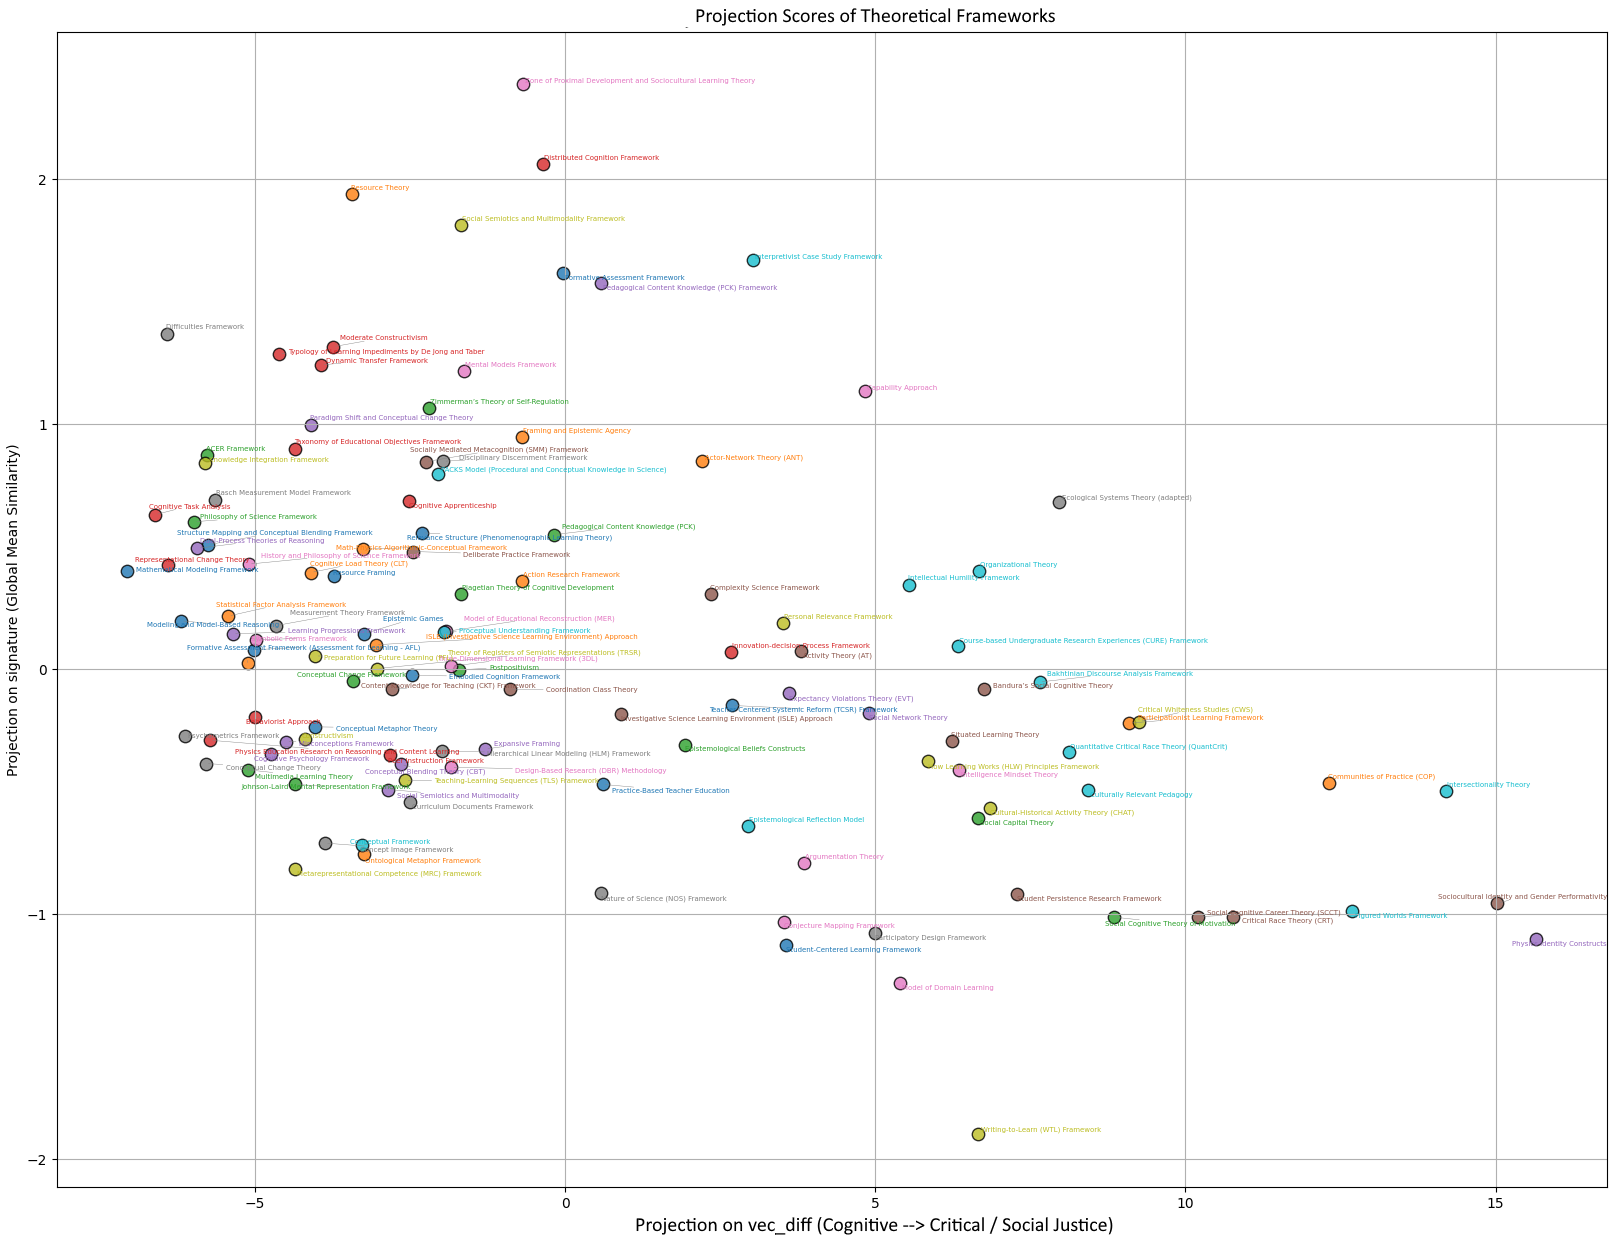
\includegraphics[width=1\linewidth]{media/theoretical_frameworks_socio_cognitive.png}
    \caption{2D projection scores of different theoretical frameworks, projection onto a "Cognitive/Critical" theories difference vector (x-axis) and the global average (y-axis).}
    \label{fig:109}
\end{figure}


In an attempt to make this sorting more rigorous we trained the previously developed projection models on this "Cogntive/Critical" theories difference vector and their respective class means. Applying the resulting classification model to the data, we saw a seemingly logical correlation between the theoretical framework and model classification of it as belonging more to either class 1 or 2 (see \Cref{tab:111}). In future work, it might be interesting to further explore whether a more sophisticated derivation of this method could be used to systematically group data based on certain semantic traits.

\begin{table}[h!]
\centering
\caption{Categorization of Theoretical Frameworks}
\begin{tabular}{|p{7cm}|p{7cm}|}
\hline
\textbf{Class 1 (Cogntive/Mathematical)} & \textbf{Class 2 (Critical/Social)} \\
\hline
Basch Measurement Model Framework & Physics Identity Constructs \\
Cognitive Task Analysis & Writing to Learn Framework \\
History and Philosophy of Science Education & Intersectionality Theory \\
Statistical Factor Analysis Framework & Sociocultural Identity and Gender Performativity \\
Constructivism & Social Cognitive Career Theory \\
Resource Framing & Student Persistence Research Framework \\
Cognitive Apprenticeships & Bandura's Social Cognitive Theory \\
Framing and Epistemic Agency & Social Capital Theory \\
Mathmatical Modeling Framework & Cultural-Historical Activity Theory \\
Multimedia Learning Theory & Quantitative Critical Race Theory \\
\hline
\end{tabular}
\label{tab:111}
\end{table}
\noindent (see notebook '2D\_projection\_space.ipynb' for implementation and further details.)
\subsection{Identifying Temporal Patterns}
Focusing in on specific theoretical frameworks, we attempt to identify temporal patterns by taking the mean embedding of all theories in the first and last year of publishing, and projecting all samples on the difference of the means. Looking at \Cref{fig:110} and \Cref{fig:111}, this approach does not seem to capture any clear linear development of the frameworks over time. While theories published in the same year seem to cluster together, the clusters jump sporadically around the x-axis from year to year rather than follow a clear incremental path from left to right over time (compared to \Cref{fig:108}). This could perhaps indicate that theories are developed in an irregular, unpredictable fashion, rather than a continuous incremental evolution. This being said, a lot of information is lost while projecting the embeddings, and it is entirely possible that a better suited difference vector could reveal a clearer pattern or trajectory.
\begin{figure}%[h!]
    \centering
    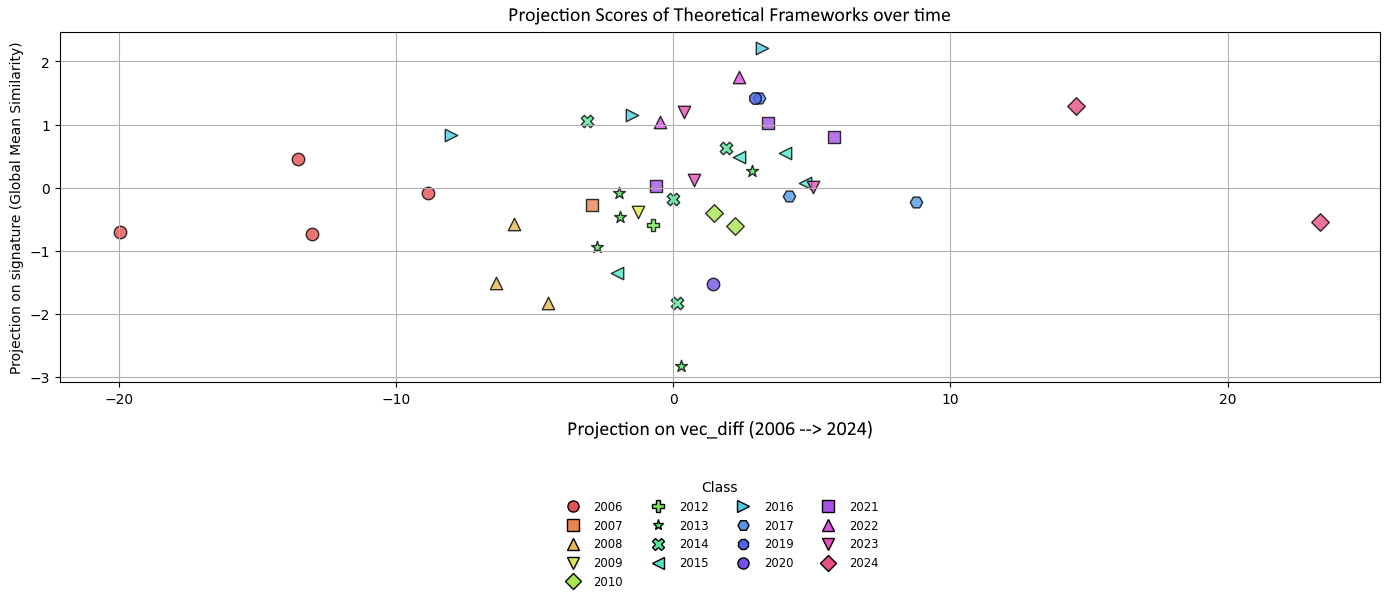
\includegraphics[width=.9\linewidth]{media/resource_framing_temporal.png}
    \caption{Projection scores of all theories classified as "Resource Framing", with 'vec\_diff' being vector difference between mean of years 2024 and 2006.}
    \label{fig:110}
\end{figure}

\begin{figure}%[h!]
    \centering
    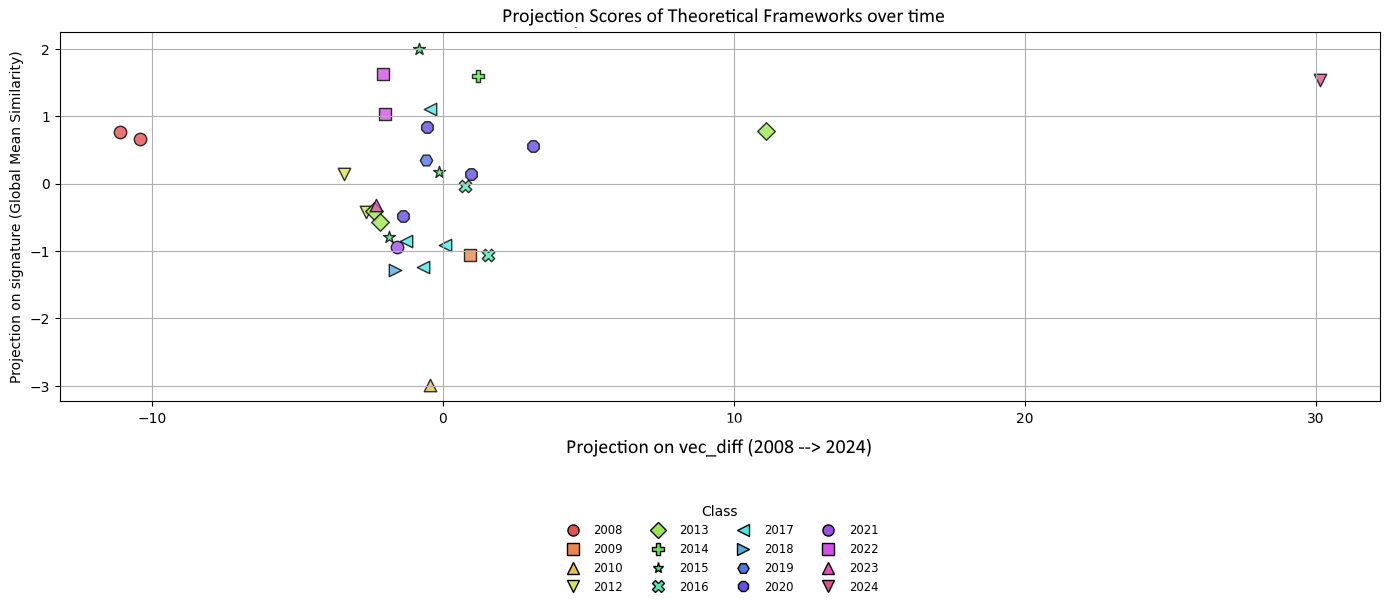
\includegraphics[width=.9\linewidth]{media/modeling_temporal.png}
    \caption{Projection scores of all theories classified as "Modeling and Model-based reasoning", with 'vec\_diff' being vector difference between mean of years 2024 and 2008.}
    \label{fig:111}
\end{figure}

\subsection{Exploring semantic correlations with article citation performance}

Using SemanticScholars API to retrieve citation counts for all the theoretical frameworks, we also attempted to look for correlations between semantic properties and average citations/yr. Dividing the theoretical frameworks into eight quantiles ranging from least to most average citations per year and projecting onto a difference vector based on the means of the highest and lowest quantiles (\Cref{fig:112}), we were unable to find any patterns or general seperation.


\begin{figure}
    \centering
    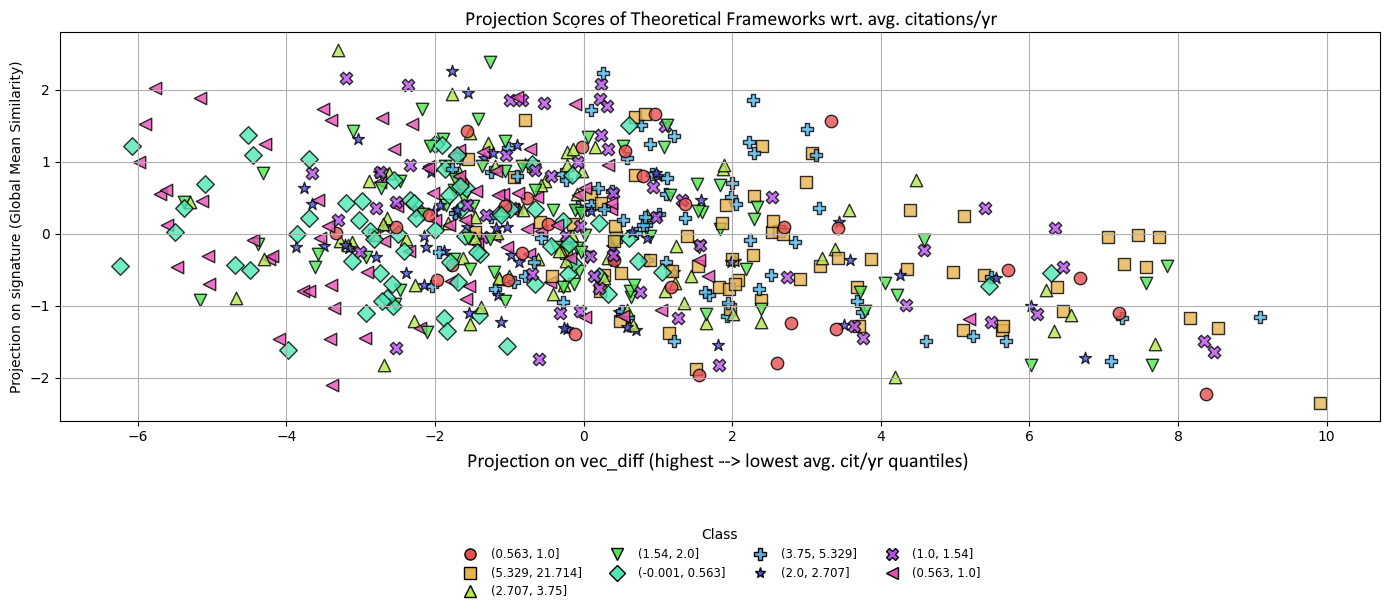
\includegraphics[width=.9\linewidth]{media/avgcityr_all.png}
    \caption{Projection scores of all theories onto difference vector between top and bottom 1/6 quantile of citations per year (x-axis) and global average embedding (y-axis). Points are labeled by their respective citations/year interval.}
    \label{fig:112}
\end{figure}
 We did however see a clear seperation between the lowest and highest citation quantiles (\Cref{fig:113}). Training our MLP projection model on this binary problem using a 0.7/0.3 train-test-split, it performs with an accuracy of $\sim$0.76. This indicates that there exists some semantic characteristic differentiating high- and low-traction academic papers.
\begin{figure}
    \centering
    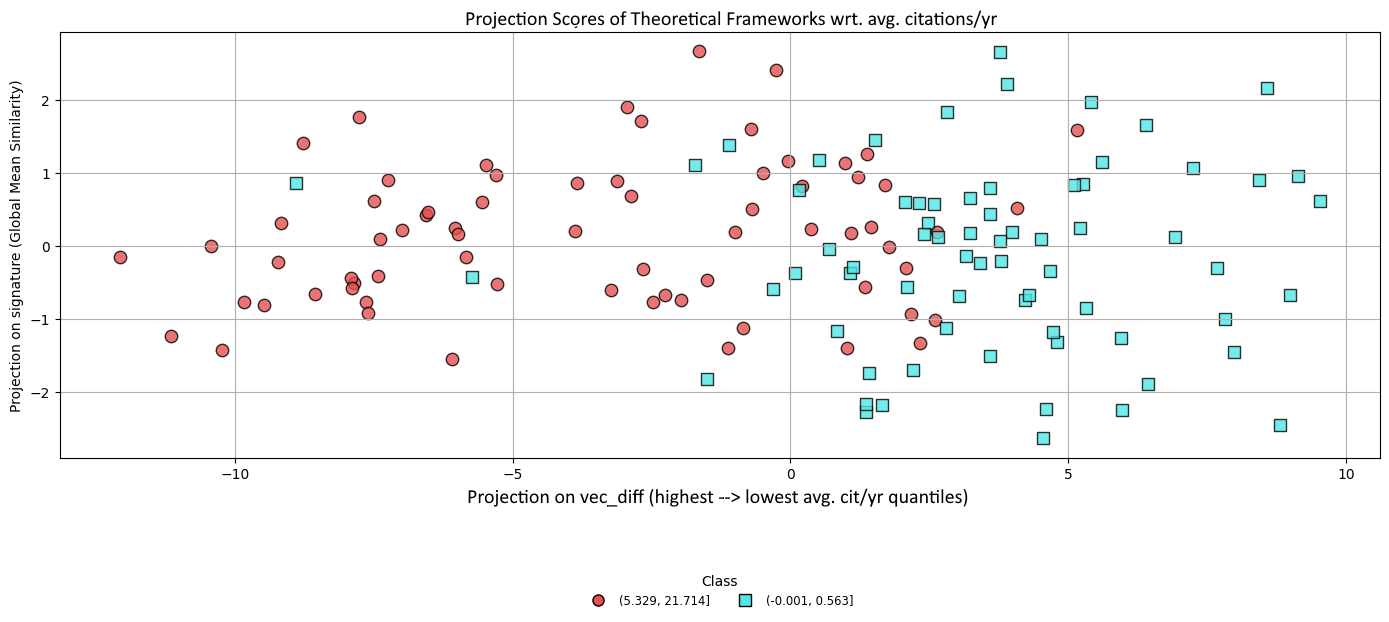
\includegraphics[width=.9\linewidth]{media/avgcityr_binary.png}
    \caption{Projection scores of all theories onto difference vector between top and bottom 1/6 quantile of citations per year (x-axis) and global average embedding (y-axis). Points are labeled by their respective citations/year interval. Here we only include points belonging to the bottom and top quantile.}
    \label{fig:113}
\end{figure}
Attempting to determine whether this semantic difference is related to the underlying nature of the theoretical frameworks, we again project the samples onto the aforementioned "Cognitive/Critical" difference vector, labeling each point by their citation performance. Looking at \Cref{fig:114}, there does not seem to be a particularly noticable crowding of either low- or high-citation papers on either the "social/critical" or "cognitive/mathematical" side, perhaps indicating that this differentiating semantic property is not dependent on theoretical orientation. Of course, this type of "visual" analysis is very "hand-wavey" and lacking in rigour, so these results should be taken with many a grain of salt.
\begin{figure}
    \centering
    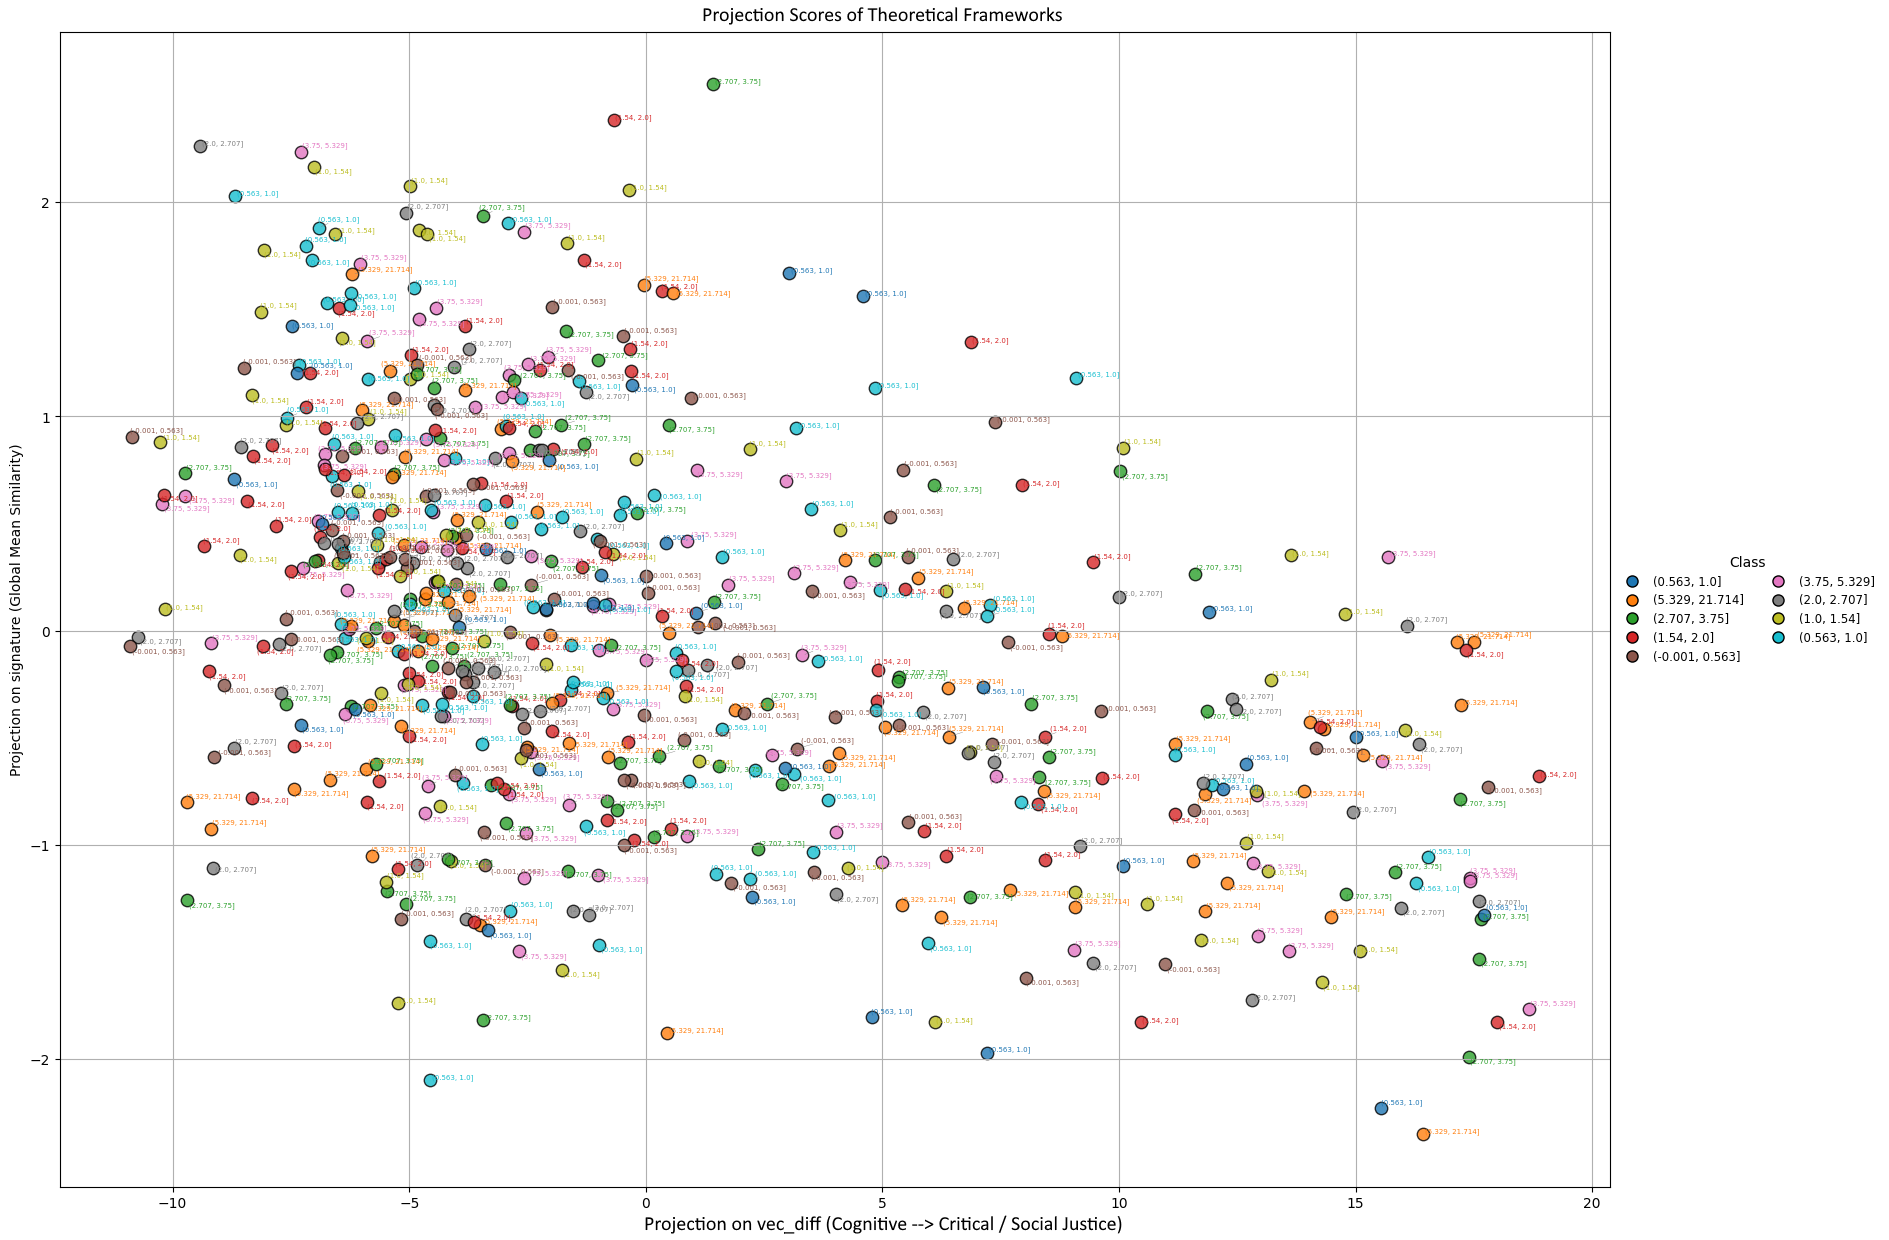
\includegraphics[width=1\linewidth]{media/cogn_crit_proj_citations.png}
    \caption{2D projection scores of theoretical framework embeddings onto "Cogntive/Critical" difference vector (x-axis) and global average (y-axis). The points are labeled according to their citations/year quantile.}
    \label{fig:114}
\end{figure}

\subsection{Discussion and Future Work}

This type of projection-based analysis, primarily centered on vector differences between mean embeddings, is conceptually intuitive and easy to implement. The general idea of substracting mean centroids to produce customized interpretable axes seems to have some merit, yielding results that align with plausable groupings. The low computational cost and high data-efficiency allows for rapid iteration and testing of different grouping hypothesis. The method is also very generalizable, and swapping the constituent centroids of the difference vector immediately changed the result sample layout in understandable ways. This flexibility could make it a useful exploratory tool.

However, the success of this method hinges almost entirely on the usefulness of the chosen difference vector. Selecting representative anchors for each conceptual pole is also a subjective process and could easily bias the outcome. Furthermore, semantic centroids flatten all internal variation within a category, and projecting all embeddings down into a 2D space may be conceptually easy to interpret, but this comes at the cost of signficant information loss that is difficult to account for. And while the results may appear conceptually straightforward, this can be misleading; these geometric operations occur in highly abstract, high-dimensional spaces, and their outcomes are not always as semantically meaningful as they might initially seem. Lastly, unlike clustering or supervised classification where evaluation metrics can guide interpretation, projection maps rely heavily on visual inspection. This makes it difficult to rigorously assess what a pattern means, or whether it’s meaningful at all.


While this analysis demontrates the potential of the projection-based semantic approach, it raises many questions and directions for future study. Further work is required to identify what the projection space captures in general. While the method is efficient and visually intuitive, interpretability of the axes remains a challenge. Although the citation difference vector successfully seperates highly and sparsely cited papers, its semantic signficant remains unclear; does it reflect alignment with theoretical paradigms, or is it more sensitive to shallow lexical and grammatical properties? Can any insights be derived from the relationship between x- and y-axes? Shedding light on these areas may also aid in the identification of temporal difference vectors that more clearly capture patterns over time. Investigating how different pre-trained models, embedding granularities, or normalization techniques affect projection behavior may also help interpret the semantic dimensions being encoded.


Developing or utilizing more rigorous inspection tools is also essential. Currently the analysis relies solely on visual inspection of plots, which is prone to inaccuracy and subjective bias. It would also be interesting to explore whether similar tools, in conjunction with a more sophisticated derivation of this method, could be used to systematically group data based on certain semantic traits. This would perhaps allow for other interesting prospects, such as the identification of emerging theoretical frameworks or under-cited but semantically novel work.